\documentclass[french]{beamer}

\usetheme{Warsaw}

\usepackage[french]{mathlist}

\usepackage[frenchb]{babel}
\usepackage[utf8]{inputenc}
\usepackage{amsmath,amssymb}

\newtheorem{defi}{Définition}
\newtheorem{theo}{Théorème}
\newtheorem{coro}{Corollaire}
\newtheorem{lem}{Lemme}

\usepackage{epic,eepic}
\usepackage{pstricks, pst-tree}

\usepackage{times}

\usepackage{ulem}

\usepackage{listings}
%\topmargin=-0.6in
\lstloadlanguages{C++}
\lstset{language=C++}
%%}

\setbeamercovered{dynamic}

\def\bxi{\boldsymbol\xi}
\def\bepsilon{\boldsymbol\epsilon}
\def\bomega{\boldsymbol\omega}
\def\aff{\operatorname{aff}}

\newcommand{\tim}[1]{\;\; \mbox{#1} \;\;}

\title[Méthodes adaptatives]{Programmation stochastique\\SAA: méthodes adaptatives}

\author{Fabian Bastin}

\date{IFT-6512 -- Hiver 2016}

\begin{document}

\frame{\titlepage}

\begin{frame}
\frametitle{Motivation}

\underline{Rappel}: nous considérons le problème stochastique
\[
{\red \min_{z \in S} g(z) = E_P \left[ G(z, \bxi) \right]},
\]
où $z \in \rit^m$ est un vecteur de variables de décision, $S$ est un
sous-ensemble compact de $\rit^m$ représentant les solutions
réalisables du problème ci-dessus, $\bxi$ est un vecteur aléatoire
réel défini sur l'espace de probabilité $( \Xi, \mathcal{F}, P )$ et
prenant des valeurs dans $( \rit^k, \mathcal{B}^k )$ ($\mathcal{B}^k$
est la mesure de Borel),
$G: \rit^m \times \rit^k \rightarrow \rit$ est une fonction à valeurs
réelles, et $E_P[\cdot]$ est l'espérance par rapport à la mesure $P$.

\mbox{}

Approximation par moyenne échantillonnale:
\[
\min_{z \in S} \hat{g}_N(z) = \frac{1}{N} \sum_{i = 1}^N G (z, \xi_i),
\]

\end{frame}

\begin{frame}
\frametitle{Convergence}

On a vu des résultats de consistence pour $N \rightarrow \infty$.
De plus, le théorème de la limite centrale nous dit que, si les tirs
sont indépendants et identiquement distribués (i.i.d.) (et $g(x)$ fini),
\[
\frac{1}{\sqrt{N}} [ \hat{g}_N(x) - g(x) ] \Rightarrow N(0, \sigma^2(x)),
\]
où $\sigma^2(x) = \mbox{var}(G(x,\xi))$, et $\Rightarrow$ dénote la
convergence en probabilité.

\mbox{}

Le résultat ci-dessus n'est valide que pour $x$ fixé.
Il est nécessaire de poser de plus fortes conditions pour avoir une
convergence fonctionnelle.

\mbox{}

Remarquons tout d'abord que sous nos hypothèses de travail,
$\hat{g}_N(x)$ est continue sur $S$, et donc peut être considéré comme
un point dans l'espace de Banach $C(s)$.

\end{frame}

\begin{frame}
\frametitle{L'espace de Banach $C(s)$}

$C(S)$ est l'espace des fonction continues $\psi: S \rightarrow \rit$,
équipé de la norme sup $\| \psi \| := \sup_{x \in S}| \psi |$

\mbox{}

$C(S)$ est un espace de Banach.
Un espace de Banach est un espace vectoriel normé complet pour la
distance issue de sa norme.
un espace métrique $M$ est dit complet ou espace complet si toute
suite de Cauchy de $M$ a une limite dans $M$ (c'est-à-dire qu'elle
converge dans $M$).

\mbox{}

On va étendre le théorème de la limite centrale (en un point) à un
théorème de la limite centrale fonctionnelle), en supposant comme
toujours que les tirs sont i.i.d.

\mbox{}

\end{frame}

\begin{frame}
\frametitle{Théorème de la limite centrale fonctionnelle}

Supposons que les conditions suivantes tiennent:
\begin{enumerate}
\item
Pour tout $x \in S$, la fonction $G(x,\cdot)$ est mesurable (autrement
dit, son espérance existe).
\item
Pour un certain point $\overline{x} \in S$, l'espérance
$E_P[G(\overline{x}, \xi)^2]$ est finie.
\item
La condition de continuité de Lipschitz
\[
| G(x_1, \xi) + G(x_2, \xi) )| \leq K(\xi) \| x_1 - x_2\|,
\]
pour une variable aléatoire à valeurs positives $K(\xi)$ telle que
$E[K(\xi)]$ est finie, tient pour tout $x_1$, $x_2 \in S$ et presque
tout $\xi$.
De plus, nous supposons que la variable aléatoire $K(\xi)$ a un moment
de second ordre fini.
\end{enumerate}

\end{frame}

\begin{frame}
\frametitle{Théorème de la limite centrale fonctionnelle (2)}

Dans ces conditions,
\[
N^{1/2} [\hat{g}_n - g] \rightarrow Y \in C(S).
\]
Avec la condition i.i.d., $Y$ est tel que pour n'importe quels points
$x_1,\ldots,x_k \in S$, le vecteur aléatoire
$(Y(x_1),\ldots,Y(x_k))^T$ a une distribution normale multivariée
de matrice de covariance donnée par la matrice de convariance du
vecteur $(G(x_1, \xi), \ldots, G(x_k, \xi))$.

\mbox{}

Dans le cas d'une minimisation globale, nous avons le résultat
suivant.
Si $N^{1/2}(\hat{g}_N - g) \Rightarrow Y \in C(S)$ (avec $\lbrace
\hat{g}_n \rbrace$ et $g$ dans $C(S)$, alors,
\[
N^{1/2}(\hat{v}_N - v^*) \Rightarrow \min_{x \in S^*} Y(x).
\]
où
\[
\hat{v}_N = \min_{x \in S} \hat{g}_N(x) \mbox{ et } v^*= \min_{x \in S} g(x).
\]

\end{frame}

\begin{frame}
\frametitle{Convergence des solutions globales}
Si $S^*$ est un singleton, dans le cas i.i.d. et les conditions
précédentes,
\[
N^{1/2}(\hat{v}_n - v^*) \Rightarrow N(0, \sigma^2(x^*) ).
\]

\mbox{}

Sous certaines conditions supplémentaires, nous avons aussi la
convergence de $E[\hat{v}_N]$ vers $v^*$.

\mbox{}

Mais tous ses résultats deviennent difficiles à étendre pour le cas
d'une optimisation locale.

\end{frame}

\begin{frame}
\frametitle{Convergence des solutions globales (2)}

Néanmoins, et c'était prévu, nous voyons que plus $N$ est grand, plus
nous devrions avoir un résultat précis. Mais plus $N$ est grand, plus
calculer la fonction approximative est coûteux, vu que
\[
\hat{g}_N(z) = \frac{1}{N} \sum_{i = 1}^N G (z, \xi_i).
\]

\mbox{}

Qu'est-ce qui nous intéresse?
\[
{\red \min_{z \in S}}\ \hat{g}_N(z) = \frac{1}{N} \sum_{i = 1}^N G (z, \xi_i).
\]
Autrement dit, pour un niveau donné d'approximation, défini par le
nombre de tirs aléatoires, il est possible d'accélérer les premiers
itérés au cours de la procédure d'optimisation en considérant des
sous-ensembles de l'échantillonnage.\\

\end{frame}

\begin{frame}
\frametitle{Méthode adaptative externe}

Alternativement, on peut commencer avec un faible échantillon et
l'étendre des itérations: 
la procédure d'échantillonnage adaptatif peut être {\blue externe} à
l'algorithme, ou {\blue interne}.
\\
Il y a donc {\red plusieurs stratégies possibles.}

\mbox{}

Une approche externe consiste à appliquer l'algorithme d'optimisation
de façon répétée avec des échantillons de tailles croissantes, comme
exprimé ci-dessous.
\begin{description}
\item[Etape 0.] Poser $k = 0$, $N_{\max}$ et $N_0$, avec $0 <
N_0 \leq N_{\max}$. Définir un certain point réalisable $\tilde{z}$.
\item[Etape 1.] Résoudre (approximativement) $\hat{g}_{N_k}$ avec
  $\tilde{z}$ comme point de départ et soit $z^*_{N_k}$ la solution
  obtenue.
\item[Etape 2.] Si $N_k = N_{\max}$, arrêt. Sinon, poser $N_{k+1}$ tel
  que $N_k < N_{k+1} < N_{\max}$, et $\tilde{z} = z^*_{N_k}$.
Incrémenter $k$ et retour à l'étape Step~1.
\end{description}

\end{frame}

\begin{frame}
\frametitle{Méthode adaptative externe - interne}

La difficulté majeure de cette procédure est de quantifier le mot
"approximatif" de l'Etape~1.
Si aucun soin n'est pris, l'algorithme résultant peut en fait
consommer plus de temps que la minimisation directe de
$\hat{g}_{N_{\max}}$.

On peut aussi remplacer le critère d'arrêt sur $N_{\max}$ par un test
d'hypothèse sur les conditions de criticalité (actuellement, seul le
premier ordre a été considéré).

\mbox{}

L'{\blue approche interne} est une stratégie non-monotone, dépendante
de la méthode d'optimisation sous-jacente.
Nous considérerons ici le cas sans contraintes.

\mbox{}

Plus précisément, générons un échantillon avant le processus
d'optimisation, avec $N_{\max}$ tirs aléatoires i.i.d.
A L'itération $k$, nous utiliserons un sous-ensemble de cette
échantillonnage initial, en utilisant $N_k$ des $N_{\max}$ tirs
aléatoires.

\end{frame}

\begin{frame}
\frametitle{Détermination de la précision}

Pour la simplicité, nous utiliserons les $N_k$ premiers tirs
aléatoires.
Ceci implique dès lors que $\hat{g}_N$ est une fonction douce bien
définie pour chaque choix de $N$.

\mbox{}

Afin de déterminer une taille d'échantillonnage, il convient de
mesurer la précision de l'approximation.
Soit $\alpha_{\delta}$ le quantile d'une $N(0,1)$
associé à un certain degré de signification $\delta$, i.e.
$P_{\bxi} [ -\alpha_{\delta} \leq X \leq \alpha_{\delta} ] = \delta$,
où $X \sim N(0,1)$.

\mbox{}

Nous utiliserons le théorème de la limite centrale,
\[
g(z) - \hat{g}_N(z) \Rightarrow N \left( 0, \frac{\sigma^2(z)}{N} \right),
\]
où $\sigma^2(z)$ est la variance de $g$ en $z$, pour construire un
intervalle de confiance pour $g(z)$ autour de $\hat{g}_N(z)$ est
\[
[\hat{g}_N(z) - \epsilon^{\delta}_N(z),\ \hat{g}_N(z) + \epsilon^{\delta}_N(z)],
\]

\end{frame}

\begin{frame}
\frametitle{Détermination de la précision (2)}

$\epsilon^{\delta}_N(z)$ est donné par
\[
\epsilon_{\delta}^N(z) = \alpha_{\delta} \frac{\sigma(z)}{\sqrt{N}}.
\]

\mbox{}

Typiquement, on choisira $\alpha_{0.9} \approx 1.64$ ou $\alpha_{0.95}
\approx 1.96$.

\mbox{}

En pratique, nous ne connaissons pas $\sigma^2(z)$, aussi nous
l'approximerons par son estimateur
\[
\hat{\sigma}^2_N(z) = \frac{1}{N-1}\sum_{i = 1}^N ( G(z,\xi_i) -
\hat{g}_N(z))^2.
\]

\mbox{}

Nous allons exploiter cette estimation de l'erreur dans le contexte
des régions de confiance.

\end{frame}

\begin{frame}
\frametitle{Principes de base}

L'idée de base est que si le modèle approxime bien la fonction
objectif par rapport à la précision de la fonction objectif elle-même
(qui est dépendante de la taille d'échantillonnage), nous présumons
que nous pourrions travailler avec une approximation moins précise et
dès lors réduire la taille de la taille d'échantillonnage.

\mbox{}

D'autre part, si l'adéquation du modèle est pauvre par rapport à la
précision de la fonction objectif, nous pouvons augmenter la taille
d'échantillonnage dans une tentative de corriger cette déficience.

\mbox{}

Nous supposons que les hypothèses exposées lors de l'analyse de
consistance tiennent.

\mbox{}

Une description formelle de l'algorithme suit.

\end{frame}

\begin{frame}
\frametitle{Algorithme: BTRDA}

Algorithme de région de confiance à précision variable.

\mbox{}

\begin{description}
\item[Etape 0. Initialisation.]
Un point initial $z_0$ et un rayon de région de confiance initial
$\Delta_0$ sont donnés.
Soit des constantes $\eta_1$ et $\eta_2$ telles que $0 < \eta_1 \leq
\eta_2 < 1$ (par exemple, $\eta_1 = 0.01$ et $\eta_2 = 0.75$).

Définissons un nombre minimum de tirs $N_{\min} = N^0_{\min}$ et une
taille d'échantillonnage $N_0$ satisfaisant $\| \nabla_{\theta}
\hat{g}_{N_0} (z_0) \| \ne 0$ si $\epsilon_{\delta}^{N_0}(z_{k+1}) \ne
0$, excepté si $N_0 = N_{\max}$.
Calculons $\hat{g}_{N_0}(z_0)$ et posons $k = 0$, $t = 0$.
\item[Etape 1. Test d'arrêt.]
Arrêt si $\| \nabla_{\theta} \hat{g}_{N_{k}}(z_{k})\| = 0$ et soit
$N_k = N_{\max}$, soit $\epsilon_{\delta}^{N_k}(z_k) = 0$.
Autrement, aller à l'Etape 2.
\end{description}

\end{frame}

\begin{frame}
\frametitle{Algorithme: BTRDA (2)}

\begin{description}
\item[Etape 2. Définition du modèle.]
Définissons un modèle $m_k^{N_k}$ de $\hat{g}_{N_k}(\theta)$ dans
$\mathcal{B}_k$.
Calculons une nouvelle taille adéquate d'échantillonnage $N^{+}$, et
posons $N^- = N_k$.
\item[Etape 3. Calcul du pas.]
Calculons un pas $s_k$ qui réduit suffisamment le modèle $m_k^{N_k}$
et tel que $z_k + s_k \in \mathcal{B}_k$.
Posons
\[ \Delta m_k^{N_k} = m_k^{N_k}(z_k) - m_k^{N_k}(z_k+s_k). \]
\item[Etape 4. Comparaison des décroissances.]
Calculons $\hat{g}_{N^+} (z_k + s_k)$ et définissons
\[
\rho_k = \frac{\hat{g}_{N_k}(z_k) - \hat{g}_{N^+}(z_k+s_k)}
{\Delta m_k^{N_k}}.
\]
\end{description}

\end{frame}

\begin{frame}
\frametitle{Algorithme: BTRDA (3)}

\begin{description}
\item[Etape 5. Mise à jour de la taille d'échantillonnage.]
Si $\rho_k < \eta_1$ et $N_k \ne N^+$, modifions $N^-$ ou la taille
d'échantillonnage candidate $N^+$ afin de prendre en compte des
différences de variance.
Recalculons $\rho_k$.
\item[Etape 6. Acceptation du point d'essai.]
Si $\rho_k < \eta_1$, definissons $z_{k+1} = z_k$, $N_{k+1} = N^-$.
Sinon, définissons $z_{k+1} = z_k + s_k$ et posons $N_{k+1} = N^+$;
incrementons $t$.

Si $N_{k+1} \ne N^{\max}$, $\| \nabla_{\theta}
\hat{g}_{N_{k+1}}(z_{k+1})\| = 0$, et
$\epsilon_{\delta}^{N_{k+1}}(z_{k+1}) \ne 0$, augmentons $N_{k+1}$ à
une certaine taille inférieure ou égale à $N_{\max}$ telle que $\|
\nabla_{\theta} \hat{g}_{N_{k+1}}(z_{k+1})\| \ne 0$ si $N_{k+1} \ne
N_{\max}$, et calculons $\hat{g}_{N_{k+1}}(z_{k+1})$.
\end{description}

\end{frame}

\begin{frame}
\frametitle{Algorithme: BTRDA (4)}

\begin{description}
\item[Etape 6. Acceptation du point d'essai (suite).]
Si $N_k = N_{k+1}$ ou si une décroissante suffisante a été observée
depuis la dernière évaluation de $\hat{g}_{N_{k+1}}$, posons
$N_{\min}^{k+1} = N_{\min}^k$.
Sinon, définissons $N_{\min}^{k+1} > N^k_{\min}$.

\item[Etape 7. Mise à jour du rayon de la région de confiance.]
\[
\Delta_{k+1} \in \begin{cases}
[\Delta_k, \infty) & \mbox{si } \rho_k \geq \eta_2, \\
[\gamma_2 \Delta_k, \Delta_k] & \mbox{si } \rho_k \in [\eta_1, \eta_2),\\
[\gamma_1 \Delta_k, \gamma_2 \Delta_k] & \mbox{si } \rho_k < \eta_1,
\end{cases}
\]
\end{description}

\mbox{}

Dans cet algorithme, la variable $t$ est utilisé pour comptabiliser le
nombre d'itérations réussies.

\mbox{}

Remarquons aussi que les algorithmes BTR et BTRDA coïncident si nous
fixons $N_k$ à $N_{\max}$ pour tout $k \geq 0$.

\end{frame}

\begin{frame}
\frametitle{Stratégie de taille d'échantillonnage variable}

Avant l'optimisation, l'utilisateur choisit une taille
d'échantillonnage maximale $N_{\max}$.
Une taille d'échantillonnage minimale $N^0_{\min}$ est définie pour
permettre l'estimation de la précision.

\mbox{}

Nous définissions aussi $N_0 = \max\lbrace N^0_{\min},
0.1N_{\max}\rbrace$ si $\| \nabla_{\theta} \hat{g}_{N_0}(z_0) \| = 0$
et $\epsilon_{\delta}^{N_0}(z_0) \ne 0$, $N_0 = N_{\max}$ sinon.

\mbox{}

Le choix de $N^+$ dans l'Etape 3 de l'algorithme BTRDA est décrit
ci-dessous.

\mbox{}

Définissons des constantes $\nu_1$ et $\chi_1$ telles que $\nu_1,
\chi_1 \in (0,1)$.
Utilisons $\epsilon_{\delta}^{N_k}(z)$ pour estimer la taille
nécessaire pour obtenir une précision égale à la décroissance du
modèle, c'est-à-dire
\[
N^s = \max \left\lbrace N^k_{\min},
\left\lceil
\frac{\alpha^2_{\delta}  \hat{\sigma}_N(z)}{(\Delta m_k^{N_k})^2}
\right\rceil \right\rbrace.
\]

\end{frame}

\begin{frame}
\frametitle{Stratégie de taille d'échantillonnage variable (2)}

Calculons le rapport entre l'amélioration du modèle et la précision estimée:
\[
\tau_1^k = \frac{\Delta m_k^{N_k}}{\epsilon_\delta^{N_k} (z_k)},
\]
et le rapport entre la taille d'échantillonnage actuelle et la taille
d'échantillonnage suggérée pour la prochaine itération:
\[
\tau_2^k = \frac{N_k}{\min \lbrace N_{\max}, N^s \rbrace}.
\]
Définissons
\[
N' =
\begin{cases}
 \min \left\lbrace \lceil \chi_1 N_{\max} \rceil, \lceil N^s
 \rceil \right\rbrace & \text{si } \tau_1^k \geq 1, \\
 \min \left\lbrace \lceil \chi_1 N_{\max} \rceil, \lceil \tau_1^kN^s
 \rceil  \right\rbrace &  \text{si } \tau_1^k < 1 \text{ et }
 \tau_1^k \geq  \tau_2^k,\\
 \lceil \chi_1 N_{\max} \rceil & \text{si }  \nu_1 \leq \tau_1^k <
 1\text{ et }\tau_1^k < \tau_2^k,\\
 N_{\max} & \text{si } \tau_1^k < \nu_1\text{ et }\tau_1^k < \tau_2^k.
\end{cases}
\]
Posons $N^+ = \max\lbrace N', N^k_{\min}\rbrace$.

\end{frame}

\begin{frame}
\frametitle{Stratégie de taille d'échantillonnage variable (3)}

Une valeur possible pour $\chi_1$ est 0.5.

\mbox{}

Si $\tau_1^k \geq 1$, la décroissance du modèle est plus grande ou
égale à la précision estimée, et nous réduisons alors la taille
d'échantillonnage au minimum entre $N^s$ et $\lceil \chi_1 N_{\max}
\rceil$.
L'idée d'utiliser $\lceil \chi_1 N_{\max} \rceil$ vient de
l'observation pratique qu'imposer une telle décroissance dans les
tailles proposées d'échantillonnage forunit une meilleure performance
numérique.

\mbox{}

Si $\tau_1^k < 1$, l'amélioration est plus petite que la précision.
Cependant, puisque l'échantillonnage a été généré avant le processus
d'optimisation, une amélioration suffisante au cours de plusieurs
itérations consécutives peut conduire à une amélioration significative
en comparaison de la précision de l'approximation, tout en gardant les
coûts de calcul plus faibles que si $N_{\max}$ tirs étaient utilisés.

\end{frame}

\begin{frame}
\frametitle{Stratégie de taille d'échantillonnage variable (4)}

Nous considérons alors deux cas.

\mbox{}

1. Si $\tau_1^k \geq \tau_2^k$, le rapport entre la taille
d'échantillonnage actuelle et la suivante potentielle est plus faible
que le rapport entre la décroissance du modèle et l'erreur estimée.
Si la taille d'échantillonnage augmente, l'erreur décroît pour un
$\Delta m_j^{N_j}$ ($j \geq k$) similaire, et dès lors $\tau_1^k$
augmente.

Nous capitalisons sur $\tau_1^k$ en calculant une taille
d'échantillonnage plus faible que $N^s$, telle qu'une amélioration de
l'ordre de $\epsilon_\delta^{N_k}(z_k)$ serait atteinte en
approximativement $\lceil \tau_1^k \rceil$ itérations si $\tau_1^j$
est similaire à $\tau_1^k$ pour $j$ proche de $k$.

Nous proposons dès lors d'utiliser le minimum entre $\lceil \chi_1
N_{\max} \rceil$ et $\lceil \tau_1^k N^s \rceil$ comme nouvelle taille
d'échantillonnage.

\end{frame}

\begin{frame}
\frametitle{Stratégie de taille d'échantillonnage variable (5)}

2. Si $\tau_1^k < \tau_2^k$, il peut néanmoins être plus économique de
continuer à travailler avec une plus petite taille d'échantillonnage,
définie à nouveau comme $\lceil \chi_1 N_{\max} \rceil$.
C'est pourquoi nous choisissons d'utiliser cette plus petite taille
d'échantillonnage aussi longtemps que $\tau_1^k$ est supérieure à un
certain seuil $\nu_1$ (par exemple 0.2).
En-deçà de ce seuil, nous considérons que la décroissance est trop
petite comparé à la précision, et nous augmentons éventuellement la
taille d'échantillonnage.

\end{frame}

\begin{frame}
\frametitle{Différences de précision}

Si $N^+$ n'est pas égal à $N_k$, le calcul de
\[
 \hat{g}_{N_k} (z_k) - \hat{g}_{N^+} ( z_k + s_k )
\]
est affecté par le changement dans la variance de l'approximation.
Ceci peut conduire à un petit rapport, voire un rapport négatif
$\rho_k$, et ce même quand le modèle $m_k^{N_k}$ donne une bonne
prédiction pour la taille d'échantillonnage $N^k$.

\mbox{}

En particulier, $\hat{g}_{N^+}(\theta)$ peut être supérieur à
$\hat{g}_{N_k}(z_k)$ pour tout $\theta$ dans un voisinage de $z_k$.
Il est dès lors important d'éviter de tels cas, ce qui motive la
possible redéfinition de $\rho_k$, comme décrit ci-après.

\end{frame}

\begin{frame}
\frametitle{Révision de la taille d'échantillonnage}

Supposons que $N_k \ne N^+$.
Si $\rho_k < \eta_1$, comparons $N^+$ et $N_k$.
Si $N^+ > N_k$, calculons $\hat{g}_{N^+}(z_k)$, $\Delta m_k^{N^+}$ et
$\epsilon_{\delta}^{N^+}(z_k)$, sinon si $N^+ < N_k$ calculons
$\hat{g}_{N_k}(z_k + s_k)$.
Posons $N^-$ à $\max\lbrace N_k, N^+ \rbrace$, et redéfinissons
\[
\rho_k = \frac{\hat{g}_{N^-}(z_k+s_k) - \hat{g}_{N^-}(z_k)}{\Delta
m_k^{N^-}}.
\]

\mbox{}

Bien que nous espérons bénéficier de plus petites tailles
d'échantillonnage quand nous sommes loin de la solution, nous devrions
être certains que nous utilisons une taille d'échantillonnage égale à
$N_{\max}$ au cours des itérations finales, afin de travailler avec la
précision voulue.
A cette fin, nous augmentons la taille d'échantillonnage minimale
quand la stratégie adaptative ne fournit pas des gains numériques
suffisants.

\end{frame}

\begin{frame}
\frametitle{Mise à jour de la taille minimale d'échantillonnage}

Nous définissons tout d'abord deux vecteurs $v$ et $l$, de dimension
$N_{\max}$, et, à l'itération $k = 0$, posons $v(N_0) =
\hat{g}_{N_0}(z_0)$, $l(N_0) = 0$, tandis que pour $i =
1,\ldots,N_{\max}$, $i \ne N_0$, posons $v(i) = +\infty$, $l(i) = -1$.

\mbox{}

Au début de l'itération $k$, $v(i) = \hat{g}_i(z_{h(i)})$, où $h(i)$
correspond à l'index de la dernière itération pour laquelle $N_{h(i)} =
i$, et $N_{h(i)-1} \ne N_{h(i)}$ si $h(i) > 0$, ou $+\infty$ si la
taille $i$ n'a pas encore été utilisée.
$l(i)$ contient le nombre d'itérations réussies jusqu'à l'itération
$h(i)$ (incluse), ou $-1$ si la taille $i$ n'a pas été utilisée.

\mbox{}

Rappel: $t$ contient le nombre total d'itérations réussies rencontrées
jusqu'à l'itération $k$ (incluse).

\end{frame}

\begin{frame}
\frametitle{Mise à jour de la taille minimale d'échantillonnage (2)}

Supposons que $N_k \ne N_{k+1}$.
Soit une constante $\gamma_3 \in (0,1]$. Si
\[
v(N_{k+1}) - \hat{g}_{N_{k+1}}(z_{k+1}) \geq
\gamma_3\nu_1(t-l(N_{k+1}))\epsilon_{\delta}^{N_{k+1}}(z_{k+1}),
\]
posons $N_{\min}^{k+1} = N_{\min}^k$.
Sinons, augmentons la taille d'échantillonnage minimale: posons
\[
N^{k+1}_{\min} \in \lbrace N_{k+1}+1,\ldots,N_{\max} \rbrace .
\]
Posons $l(N_{k+1}) = t$ et $v(N_{k+1}) = \hat{g}_{N_{k+1}}(z_{k+1})$.

\mbox{}

Une valeur pratique pour $\gamma_3$ est 0.5.
Notons que $N^{k+1}_{\min} > N^k$ si le test ci-dessus n'est pas
satisfait.

De plus, nous avons que si $N_k \ne N_{k+1}$, $t-l(N_{k+1}) \geq 1$.
Ceci est clairement vérifié si $l(N_{k+1}) = -1$, aussi sans perte de
généralité, nous supposons que $l(N_{k+1}) \geq 0$.
Au début de l'itération $k$, nous avons $l(N_i) \leq t$, $i =
1,\ldots,N_{\max}$.

\end{frame}

\begin{frame}
\frametitle{Mise à jour de la taille minimale d'échantillonnage (3)}

Si $\rho_k \geq \eta_1$, $t$ est incrémenté de $1$ au cours de
l'Etape~6 de l'algorithme de région de confiance, aussi $l(N_{k+1}) <
t$ dans l'algorithme ci-dessus.

Si $\rho_k < \eta_1$, de l'algorithme de mise à jour de la taille
d'échantillonnage, $N_k < N_{k+1}$ puisque des réductions de tailles
d'échantillonnage peuvent seulement se produire lors d'itérations
réussies. Ceci implique aussi que $l(N_{k+1}) < l(N_k) \leq t$.

\mbox{}

Finalement, notons que si $N_k \ne N_{\max}$, nous ne pouvons pas
exclure le cas pathologique dans lequel $z_k$ est un point critique au
premier ordre pour $\hat{g}_{N_k}$.

Si $\epsilon_{\delta}^{N_k}(z_k) \ne 0$, l'algorithme ne s'arrête pas,
mais puisque le modèle est quadratique, aucune décroissance n'est
atteinte si $H_k$ est défini positif.

\end{frame}

\begin{frame}
\frametitle{Précautions additionnelles}

Afin d'éviter cette situation, nous forçons dès lors une croissance de
$N_{k+1}$ quand cette situation se produit.

\mbox{}

En pratique cependant, la norme du gradient change habituellement
lentement dans un voisinage d'un tel point critique, et un petit
gradient conduit typiquement à un petite décroissance du modèle, ce
qui mène à l'augmentation de la taille d'échantillonnage et $N_{\max}$
est atteinte avant que cette précaution ne soit mise en oeuvre. 

\end{frame}

\begin{frame}
\frametitle{Convergence: en bref}

\begin{theo}
Sous certaines hypothèses de régularité, si
\[
\exists \kappa > 0\text{ such that }
\epsilon_{\delta}^{N_k}(z_k) \geq \kappa,
\]
pour tout $k$ suffisamment grand, alors, presque sûrement,
l'algorithme converge en un nombre fini d'itération avec un nombre
final de tirs aléatoires égal à $N_{\max}$, ou le nombre d'itérations
est infini et il existe un certain $j$ tel que pour toutes les
itérations $i$, $i \geq j$, $N_i$ est égal à $N_{\max}$.
\end{theo}
Preuve: voir Bastin, Cirillo et Toint, {\sl An adaptive {Monte Carlo}
  algorithm for computing mixed logit estimators}, Computational
Management Science 3(1), pp. 55--79, 2006.

\mbox{}

Nous pouvons alors prouver la convergence au premier et second ordre,
et ce pour le SAA avec $N_{\max}$ tirs.

\end{frame}

\begin{frame}
\frametitle{Exemple}

Modèle logit mélangés: maximisation de vraisemblance stochastique
\begin{center}
\psshadowbox[fillstyle=solid, fillcolor=lightgray]{
$\max_{\theta} LL(\theta) =
\max_{\theta} \frac{1}{N} \sum_{n = 1}^{N} \ln E[P_{ij_i}(x,\theta,\xi)].$
}
\end{center}

Modèle de choix de mode: données {\blue Mobidrive} (Axhausen
and al., 2002)\\
$N = 5799$ observations, $R_{\max} = 2000$ tirs par individu, 14
paramètres (dimension d'intégration: 3 variables normales).

\begin{center}
\begin{minipage}{0.49\linewidth}
\includegraphics[angle=270, width=\linewidth]{2000_sample_iter.ps}
\end{minipage}
\begin{minipage}{0.49\linewidth}
\includegraphics[angle=270, width=\linewidth]{2000_sample_fct.ps}
\end{minipage}
\end{center}
\begin{tiny}
{\red
\hspace*{6.8cm}$\downarrow$\hspace*{3cm}$\downarrow$\\
\hspace*{6.0cm}Starting value\hspace*{1.2cm}Maximum value\\
}
\end{tiny}

\end{frame}

\end{document}